% JAWS 2 @ ASE 2026 — Idea Paper (≤8 pages excl. references)
% ACM Primary Article Template, sigconf, single-anonymous
\PassOptionsToPackage{expansion=false}{microtype}
\documentclass[sigconf,nonacm]{acmart}

% JAWS is single-anonymous: author names visible
\settopmatter{authorsperrow=3}

\usepackage{booktabs}
\usepackage{multirow}
\usepackage{xcolor}
\usepackage{tikz}
\usetikzlibrary{arrows.meta,positioning,calc,decorations.pathreplacing}

% Blind-review off (single-anonymous)
\setcopyright{none}
\renewcommand\footnotetextcopyrightpermission[1]{}
\pagestyle{plain}

\title{From Symptom to Structure: Analyzing Disagreement\\in Agent-Skill Security Scanners}






\begin{abstract}
Automated security analyses routinely disagree, yet evaluations treat that disagreement as a statistic---Cohen's $\kappa$, pairwise overlap---and stop there, as if it were noise or merely an outcome about tool quality.
We propose to treat disagreement differently: as \emph{analytical evidence about the analyses themselves}.
The structure of disagreement, once made comparable, exposes each analysis's coverage of the threat space and how it operationalizes detection there.
We develop a methodology for this conversion: a shared observation language that makes disagreement localizable, a decomposition into \emph{coverage gaps} and \emph{operational divergence}, blind-spot hypotheses locked before construction, and adversarial validation.
We instantiate the idea on agent-skill security scanners, an emerging supply-chain defense whose scanners disagree sharply.
Across 582 real malicious skills and three heterogeneous scanners, the decomposition predicts concrete blind spots, and locked adversarial construction confirms them: hidden-file payloads evade SkillSpector on 14/15, expression variants evade Cisco on 6/6, and combined strategies evade SkillSpector on 5/5, with selected failures traced to source-level mechanisms.
Disagreement, we argue, is not merely a statistic to report: it is evidence to mine.
\end{abstract}

\keywords{agent skills, security scanners, taxonomy, blind spots, adversarial construction}

\begin{document}
\maketitle

% ============================================================
\section{Introduction}
\label{sec:intro}

Automated security analyses disagree.
Given the same artifact, one scanner flags it, another passes it, and a third flags something else entirely.
The standard response is to \emph{measure} the disagreement---Cohen's $\kappa$, pairwise overlap, per-tool recall---and treat the result as an evaluation outcome: a fact about tool quality, or noise to be averaged away.
We ask a different question: \emph{what does the pattern of disagreement reveal about the analyses themselves?}
We argue that disagreement is not merely a statistic to report.
It is analytical evidence: once disagreements are made comparable, their structure exposes what each analysis covers, what it cannot see, and why.

Today this evidence is inaccessible, because analyses speak incompatible languages.
One scanner reports ``tool poisoning,'' another ``supply-chain risk,'' a third a family of regex matches.
There is no shared frame in which to ask \emph{where exactly} they disagree, so disagreement remains global---a $\kappa$---but never localizable.
Without localization there is no explanation; without explanation, disagreement cannot be acted upon.

We propose to convert disagreement into structure.
The conversion has four steps.
First, a \emph{shared observation language}---a coordinate space over the threat space---into which each scanner's categories are mapped, making disagreement localizable.
Second, a \emph{structural decomposition}: localized disagreement separates into \emph{coverage gaps} (a scanner does not inspect a region at all) and \emph{operational divergence} (scanners cover the same region but instantiate detection differently).
Third, the decomposition yields \emph{blind-spot hypotheses}, which we lock before building anything.
Fourth, \emph{adversarial validation}: coordinate-driven construction tests the locked hypotheses, and selected failures are traced to implementation mechanisms.

We instantiate this idea on \emph{agent-skill security scanners}.
Coding agents extend their capabilities by installing skills---packages of instructions and scripts---and malicious skills are a live supply-chain threat (the ClawHavoc incident surfaced over 1{,}184 of them~\cite{clawhub2026}).
Scanners have emerged to screen skills, but they disagree sharply~\cite{clawhub2026,locatejudge2026}, and no existing evaluation explains the disagreement.
The object is timely; the methodology is the contribution.

An honesty point frames our results.
In aggregate the scanners are strong: across 582 real malicious skills, SkillSpector detects 92.8\%, Cisco 85.2\%, Caterpillar 72.5\%.
The blind spots are therefore invisible in average recall; they emerge only when the threat space is partitioned.
This is precisely the structure that aggregate metrics conceal, and precisely what disagreement, treated as evidence, exposes.

\noindent\textbf{Contributions.} This is an idea paper: one general claim, a methodology, an instantiation, and early evidence.
\begin{itemize}
  \item \textbf{Idea.} Disagreement among automated security analyses is analytical evidence, not merely an evaluation outcome.
  \item \textbf{Methodology.} A conversion pipeline: shared observation language $\rightarrow$ structural decomposition $\rightarrow$ locked hypotheses $\rightarrow$ adversarial validation (\S\ref{sec:measure}--\S\ref{sec:validate}).
  \item \textbf{Instantiation.} Agent-skill security scanners, studied via a three-dimensional attack-coordinate space.
  \item \textbf{Early evidence.} 582 real malicious skills, three scanners, 129 locked adversarial constructions, and source-level mechanism tracing.
\end{itemize}

\noindent\textbf{Scope.} We demonstrate the loop end-to-end on one instantiation.
The generality of the idea---to package scanners, dependency scanners, static analyzers, LLM-based security evaluators---is the research direction this early result opens, to be developed in an extended version.

\noindent\textbf{Results.} Hidden-file payloads evade SkillSpector on 14/15 samples (its build context skips dotfiles). Expression-layer variants evade Cisco on 6/6 (its pipeline requires literal command surfaces). Combined strategies evade SkillSpector on 5/5.
A regex-only reference tool is blind to all 10 semantic variants, showing blind spots deepen as detection grows more primitive.

\noindent\textbf{Paper identity.} Disagreement is not merely a number: it reveals structure that can be hypothesized about and tested.

% ============================================================
\section{Background and Motivation}
\label{sec:background}

Agent skills are distributed through marketplaces such as ClawHub and skills.sh~\cite{clawhub2026}; at scale, a snapshot of 138{,}133 public SKILL.md files found 91.8\% exhibiting at least one packaging or safety defect~\cite{reusability2026}, and field measurements attribute 26.1\% of 31{,}132 wild skills with at least one security vulnerability~\cite{skillscan2026}. Because a skill can carry arbitrary instructions and scripts, it is an active supply-chain attack surface: the ClawHavoc incident identified over 1{,}184 malicious skills in a single marketplace~\cite{clawhub2026}, and injected skill instructions achieve up to 80\% attack success on frontier agents~\cite{skillinject2026}. Security scanners have emerged to screen skills before installation~\cite{locatejudge2026}.

We study three scanners spanning the mainstream detection architectures (Table~\ref{tab:scanners}). \textbf{SkillSpector} (NVIDIA) combines static rules, AST analysis, YARA signatures, and an LLM semantic layer. \textbf{Cisco Skill Scanner} (AI Defense) combines static analysis, YARA, LLM-based judgment, and behavioral dataflow. \textbf{Caterpillar} is a lightweight regex-based tool. SkillSpector and Cisco are production-grade; Caterpillar serves as a lower-bound reference showing how blind spots deepen as detection grows more primitive. The three decision rules already preview the operational divergence that \S\ref{sec:explain} measures: a numeric risk score, a severity threshold, and a lexical grade.

\begin{table}[t]
\caption{The three studied scanners. ``Decision rule'' is what the raw output reduces to for an allow/block decision: each rule is later implicated in a distinct blind spot.}
\label{tab:scanners}
\small
\begin{tabular}{@{}p{1.5cm}p{2.6cm}p{3.6cm}@{}}
\toprule
Scanner & Layers & Decision rule \\
\midrule
SkillSpector & static rules, AST, YARA, LLM semantic & risk score (0--100); $>$50 = detected \\
Cisco & static, YARA, LLM judgment, dataflow & safe unless a CRITICAL/HIGH finding exists \\
Caterpillar & regex families & letter grade; $\neq$A = flagged \\
\bottomrule
\end{tabular}
\end{table}

\textbf{Threat model.} The attacker authors and publishes a skill that a user (or an agent acting for the user) installs from a marketplace. The skill may contain natural-language instructions in SKILL.md, arbitrary scripts, and metadata declarations; everything is readable, but nothing is executed at install time. The defender runs one or more scanners over the skill \emph{before} execution and must decide allow/block with no runtime evidence. The attacker's goal is not to exploit a parser bug but to place malicious behavior where the defender's analysis does not look: outside the scanned file set, outside the literal command surface, or inside a declared capability. All blind spots we report are of this placement kind: architectural, not cryptographic.

These scanners frequently disagree on the same skill. Recent measurements quantify the disagreement: across 67{,}453 skills, pairwise overlap of flagged sets is at most 10.4\%, and only 0.69\% are flagged by all scanners~\cite{clawhub2026}. Yet such numbers stay descriptive: they tell us \emph{that} scanners disagree, not \emph{where} in the attack space the disagreement arises or \emph{why}.

% ============================================================
\section{A Shared Observation Language}
\label{sec:measure}

The reason disagreement cannot currently be interrogated is that the scanners speak incompatible languages: SkillSpector speaks of 17 risk classes, Cisco of 18 threat categories, Caterpillar of regex rule families. There is no frame in which to ask \emph{where exactly} they disagree. The coordinate space we introduce is, first and foremost, a \emph{shared observation language}: the instrument that makes disagreement localizable. It is not a universal taxonomy; it is the observation layer required to interrogate disagreement. Figure~\ref{fig:pipeline} shows the full conversion this paper instantiates.

\begin{figure*}[t]
\centering
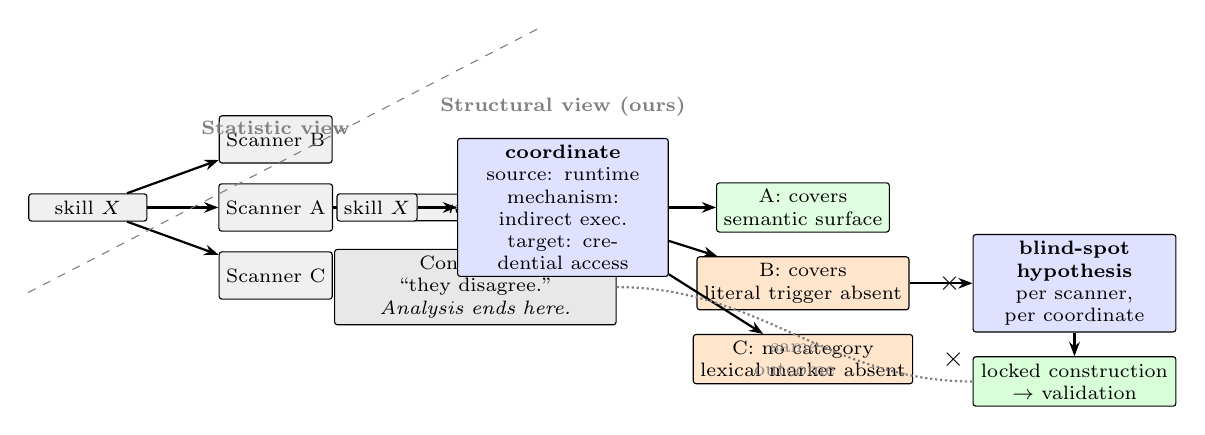
\begin{tikzpicture}[node distance=3mm and 5mm,
  box/.style={draw, rounded corners=1pt, font=\scriptsize, align=center, inner sep=2.5pt},
  arrow/.style={-{Stealth[length=1.8mm]}, thick},
  scan/.style={draw, rounded corners=1pt, font=\scriptsize, align=center, inner sep=2.5pt, minimum width=13mm, minimum height=6mm}]

% ---- LEFT: statistic view ----
\node[box, fill=gray!12, minimum width=15mm] (skill) {skill~$X$};
\node[scan, right=9mm of skill, fill=gray!12] (sa) {Scanner A};
\node[scan, above=2.5mm of sa, fill=gray!12] (sb) {Scanner B};
\node[scan, below=2.5mm of sa, fill=gray!12] (sc) {Scanner C};
\draw[arrow] (skill) -- (sb); \draw[arrow] (skill) -- (sa); \draw[arrow] (skill) -- (sc);
\node[right=2.5mm of sb] {$\checkmark$};
\node[right=2.5mm of sa] {$\times$};
\node[right=2.5mm of sc] {$\times$};
\node[box, right=10mm of sa, fill=gray!12, minimum width=16mm] (kappa) {$\kappa \approx 0$};
\draw[arrow] (sa) -- (kappa);
\node[box, below=3.5mm of kappa, fill=gray!18, text width=34mm] (end1) {Conclusion: ``they disagree.''\\ \emph{Analysis ends here.}};
\draw[arrow] (kappa) -- (end1);

% ---- divider ----
\draw[dashed, gray] ($(skill.south west)+(0,-9mm)$) -- ($(kappa.north east)+(0,21mm)$);
\node[font=\scriptsize\bfseries, gray] at ($(sa.north)+(0,7mm)$) {Statistic view};

% ---- RIGHT: structural view ----
\node[box, right=24mm of skill, fill=gray!12] (skill2) {skill~$X$};
\node[box, right=5mm of skill2, fill=blue!12, text width=25mm] (coord) {\textbf{coordinate}\\ source: runtime\\ mechanism: indirect exec.\\ target: credential access};
\draw[arrow] (skill2) -- (coord);

\node[scan, right=6mm of coord, fill=green!12] (ra) {A: covers\\ semantic surface};
\node[scan, below=3mm of ra, fill=orange!20] (rb) {B: covers\\ literal trigger absent};
\node[scan, below=3mm of rb, fill=orange!20] (rc) {C: no category\\ lexical marker absent};
\draw[arrow] (coord) -- (ra); \draw[arrow] (coord) -- (rb); \draw[arrow] (coord) -- (rc);
\node[right=2.5mm of ra] {$\checkmark$};
\node[right=2.5mm of rb] {$\times$};
\node[right=2.5mm of rc] {$\times$};

\node[box, right=8mm of rb, fill=blue!12, text width=24mm] (hyp) {\textbf{blind-spot hypothesis}\\ per scanner, per coordinate};
\draw[arrow] (rb) -- (hyp);
\node[box, below=3mm of hyp, fill=green!15, text width=24mm] (val) {locked construction\\ $\rightarrow$ validation};
\draw[arrow] (hyp) -- (val);
\node[font=\scriptsize\bfseries, gray] at ($(coord.north)+(0,4mm)$) {Structural view (ours)};

% same-result annotation
\draw[densely dotted, thick, gray] (end1.east) to[out=0,in=180] node[midway, below, font=\scriptsize, text=gray, align=center] {same\\ outcome} (val.west);
\end{tikzpicture}
\caption{\textbf{The same disagreement, read two ways.} The statistic view collapses three verdicts on skill~$X$ into a scalar and stops. The structural view localizes skill~$X$ to an attack coordinate, reads each scanner's coverage and detection surface there, derives per-scanner blind-spot hypotheses, and validates them by locked construction. Same outcome, different explanatory power.}
\label{fig:pipeline}
\end{figure*}

\begin{table}[t]
\caption{The three-dimensional observation language. Each threat is a coordinate $(source, mechanism, target)$; all three axes are multi-valued.}
\label{tab:dims}
\small
\begin{tabular}{@{}p{1.2cm}p{1.9cm}p{4.6cm}@{}}
\toprule
Dimension & Question & Values (abbreviated) \\
\midrule
source & where does it enter? & supply chain; user input; external untrusted content; runtime environment; unknown \\
mechanism & how does it attack? & code execution; instruction manipulation; dependency manipulation; privilege abuse; obfuscation; state corruption; \ldots \\
target & what does it seek? & information theft; persistent control; resource abuse; system damage; financial theft; content-safety harm; defense evasion \\
\bottomrule
\end{tabular}
\end{table}

\subsection{Three Dimensions}
Each threat is located by three dimensions (Table~\ref{tab:dims}): \emph{source} (where it enters: supply chain, user input, external untrusted content, runtime environment, or unknown), \emph{mechanism} (how it attacks: code execution, instruction manipulation, dependency manipulation, privilege abuse, obfuscation, state corruption, \ldots), and \emph{target} (what it seeks: information theft, persistent control, resource abuse, system damage, financial theft, content-safety harm, defense evasion). The axes follow established security modeling: the attacker model (cf.\ Dolev--Yao), the technique axis (cf.\ ATT\&CK), and the security-property axis (cf.\ the CIA triad).

\subsection{Mapping Scanner Languages}
We mapped 67 scanner-native categories into the space, producing 43 coordinates. The mapping is manual and evidence-based: each native category (e.g.\ Cisco's ``tool poisoning,'' SkillSpector's 17 risk classes, Caterpillar's rule families) is assigned to the set of coordinates its triggering conditions actually observe, with multi-valued assignment when a category spans several coordinates; a credential-harvesting rule, for instance, covers any (source $\times$ code execution $\times$ information theft) cell regardless of how the credential was reached. This is where ``semantic alignment'' becomes checkable: two categories from different scanners that map to overlapping coordinate sets are nominally the same detector, and any residual disagreement between them is operational, not semantic. To check that the space can carry existing threat descriptions, we mapped 1{,}253 threat statements from 84 sources. Only 17.9\% map cleanly to a full triple; \textbf{56.5\% are partial triples}: existing vocabularies cannot even fully express them, and 20.3\% fall into genuine gaps. This partial-triple rate is our key measurement-space evidence: current categorizations do not provide a complete description; a coordinate space does.

\subsection{Orthogonality}
The dimensions carry complementary information. On an 81-row human-verified gold standard, pairwise normalized mutual information is 0.565 (source$\times$mechanism), 0.492 (mechanism$\times$target), and 0.232 (source$\times$target): the axes correlate but do not collapse into each other. Ablating any single axis destroys 21\% (source), 38\% (target), or 41\% (mechanism) of coordinate resolution, and full three-dimensional coordinates resolve threats $2.6\times$ more finely than the best pair. The space therefore carries non-redundant information and serves as the observation layer for all subsequent analysis.

% ============================================================
\section{Structural Disagreement Analysis}
\label{sec:explain}

With a common observation layer in place, we project each scanner's detections onto the coordinate space and compare scanners coordinate by coordinate. This is the paper's core analysis, measured on 582 real malicious skills (350 wild samples stratified by behavior, 232 coordinate-generated).

\subsection{Aggregate Detection Conceals the Structure}
In aggregate the scanners are strong: SkillSpector detects 92.8\%, Cisco 85.2\%, Caterpillar 72.5\%. Stopping here, one would conclude detection is largely solved. The blind spots are invisible at this level of abstraction; they emerge only when the attack space is partitioned.

\subsection{Coverage Gaps}
The first structural cause of disagreement is a \emph{coverage gap}: a scanner does not inspect a coordinate at all. The per-dimension agreement pattern localizes where: after mapping the scanners' outputs to coordinates, inter-scanner agreement splits by axis: moderate on \emph{target} ($\kappa=+0.223$), near-zero on \emph{mechanism} ($-0.025$), and negative on \emph{source} ($-0.137$), because scanners report behavior, not provenance. Coordinates whose source is the runtime environment or user input are systematically less covered than supply-chain coordinates: a payload whose malice lives in a runtime dataflow (user input interpolated into a command pipeline) has no static surface in the skill text, and scanners that do not model that flow cannot see it at all.

\subsection{Operational Divergence}
The second cause is subtler. Scanners can \emph{semantically agree} that a coordinate matters while \emph{operationally diverging} on how to detect it. Consider the coordinate (credential access $\times$ code execution $\times$ data exfiltration): all three scanners nominally cover it, yet SkillSpector instantiates detection through script-level semantic evidence, Cisco through literal command triggers, and Caterpillar through lexical regex patterns. Same coordinate, same semantic intent, three different operational surfaces. An attack that removes the literal surface evades Cisco and Caterpillar while SkillSpector may still catch it, and vice versa for attacks that hide the script.

Figure~\ref{tab:forms} shows where the two production scanners' declared coverage diverges, coordinate by coordinate. The map separates two kinds of disagreement that a $\kappa$ conflates. In the 10 \emph{both-declare} coordinates, disagreement is operational: both scanners cover the region but instantiate detection differently, SkillSpector via script-level semantic evidence and Cisco via literal command triggers. An attack that removes the literal surface evades Cisco while SkillSpector may still catch it; attacks that hide the script do the reverse. In the 16+4 \emph{single-coverage} coordinates, the disagreement is a coverage gap: one scanner simply has no category that maps there. The 13 \emph{neither} coordinates are collectively unguarded by both production scanners; and the regex tool is structurally unmappable---it has no category system at all. Construction results confirm the reading: on the both-declare region, pure-instruction runtime payloads drop Cisco to 22\% while SkillSpector holds 100\%; hidden-file payloads drop SkillSpector to 27\% while remaining visible to YARA-level rules (a threshold failure, not a gap; \S\ref{sec:validate}); removing literal commands blinds the regex engine entirely (0/10) while SkillSpector is unaffected. No attack form is missed by all scanners, but no scanner survives all forms. Disagreement of this shape is not noise; it is a map of each scanner's operational surface.

\begin{figure}[t]
\centering
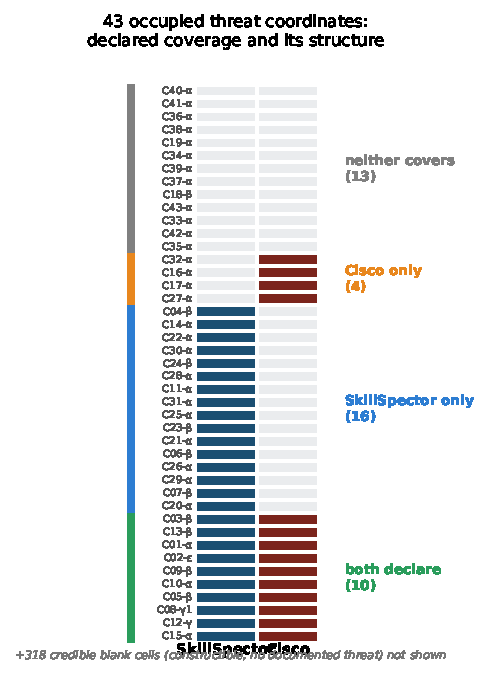
\includegraphics[width=0.92\columnwidth]{fig_structure_map.pdf}
\caption{\textbf{The structure of declared coverage across 43 occupied threat coordinates.} Rows are coordinates (IDs at left); filled cells are categories the scanner maps onto that coordinate. The four bands are four disagreement states: 10 coordinates where both production scanners declare coverage (candidate operational divergence), 16 covered only by SkillSpector, 4 only by Cisco, and 13 covered by neither (several only by external reference taxonomies). A regex tool with no category system appears in no column; it cannot be mapped at all. Color encodes \emph{disagreement type}, not detection rate.}
\label{tab:forms}
\end{figure}

\subsection{Misclassification and the Grey Zone}
A third, orthogonal finding: scanners can detect a behavior but misclassify its intent. In a pilot audit of 30 SkillSpector findings, every one described a real capability that was in fact a legitimate, declared tool behavior: ``dangerous but legal.'' Detection fired; the verdict was wrong. This is the false-positive side of the same structural story: the scanners' vocabularies have no slot for ``declared, justified capability,'' so a skill that legitimately reads credentials for its stated purpose lands in the same category as one that exfiltrates them. For governance, an unchecked false-positive rate is as corrosive as a blind spot: users disable scanners that cry wolf, and the blind spot then inherits the whole pipeline. Our decomposition treats the grey zone as a first-class object: the misclassification rate is a property of the operational divergence, not of the corpus.

% ============================================================
\section{From Analysis to Blind-Spot Hypotheses}
\label{sec:hypotheses}

The coordinate space is not itself a blind-spot oracle. It is a common observation layer through which two kinds of evidence are turned into explicit, pre-specified hypotheses, which we lock \emph{before} building any adversarial sample. To prevent post-hoc rationalization, we separate exploratory experiments from confirmatory ones.

\subsection{Two Evidence Sources}
\emph{Type A (coordinate-coverage evidence).} Projecting every mapped category onto the space yields a scanner-by-coordinate coverage matrix. The matrix makes absence explicit: of the 400 cells in the cross-product of our observed dimension values, only 43 are occupied by any documented threat, 318 are credible blanks (constructible but undocumented), and 39 are infeasible. A coordinate uncovered or weakly covered by a scanner's mapped categories yields the hypothesis that the scanner will miss attacks occupying that coordinate, and the 318 credible blanks delimit exactly where such hypotheses can be tested.

\emph{Type B (scanner-architecture evidence).} An implementation property produces a mechanistic limitation. Reading SkillSpector's source, for instance, shows that its build context skips dotfiles; this produces the hypothesis that hidden-file payloads will evade analysis.

\subsection{Sanitization: Separating Real Misses from Artifacts}
Construction experiments are easily polluted by artifacts that look like scanner misses. Our protocol applies three checks to every sample. \emph{Malice realism:} each sample is verified to contain the attack it was specified to contain: LLM generators sometimes emit a benign variant or silently drop the payload script, and a ``miss'' on such a sample is a generator artifact. \emph{Technical-failure classification:} scanner API timeouts, malformed submissions, and crashes are classified as indeterminate and excluded, never counted as misses. \emph{Ground-truth hygiene:} provenance metadata and experiment-arm prefixes are stripped before scanning, so no classifier can leak the label through the filename. The discipline is load-bearing: an early construction round appeared to show a 56\% all-scanner miss rate; after sanitization the true all-miss count was zero. Without these checks, a construction experiment measures the generator, not the scanner.

\subsection{Hypothesis-Locking Protocol}
For each hypothesis we record the evidence, the locked prediction, the construction specification, and the validation outcome. Locking precedes construction: the specification is written from the hypothesis, not from observed misses. Our timeline is explicit and reproducible: the coordinate-coverage matrix and blind-spot hypotheses were recorded on 2026-08-13; confirmatory construction began 2026-08-19. The hidden-file hypothesis, for instance, was derived by reading SkillSpector's build-context source \emph{before} any hidden-file sample existed. Arms~1--6 preceded the matrix and are labeled exploratory: they establish that coordinate-driven construction is feasible, and none of their outcomes enters the hypothesis table.

% ============================================================
\section{Early Evidence: Adversarial Validation}
\label{sec:validate}

We now demonstrate that the loop works end-to-end. This is early evidence, proof of feasibility for the idea and the methodology, rather than a claim of benchmark completeness. We validate locked hypotheses through coordinate-driven adversarial construction: 129 constructed samples across 13 experiment arms, each scanned by all three scanners.

\subsection{Centerpiece: Hidden-File Payloads}
\emph{Evidence (Type B):} SkillSpector's build context skips dotfiles. Figure~\ref{fig:oneload} traces one payload through all three scanners.
\emph{Locked hypothesis:} payloads placed in hidden files (\texttt{.env}, \texttt{.profile}) will evade SkillSpector.
\emph{Construction:} 15 skills whose SKILL.md is benign, the payload living entirely in a dotfile. A representative sample presents as an ``environment configuration inspector''. The SKILL.md instructs the agent to validate configuration hygiene. The bundled \texttt{.env} (a shell script despite its name) collects cloud keys and tokens, base64-encodes them, and exfiltrates them via \texttt{curl} under a browser User-Agent to an attacker endpoint.
\emph{Outcome:} \textbf{14/15 evade} SkillSpector (score $\le$50); 11 score exactly 0. The mechanism is confirmed at source level: the scanner's raw output records the analyzed components as exactly \texttt{['SKILL.md']}: the dotfiles never entered the scanned context. The two production scanners fail on the same samples for different reasons, which is the decomposition in action: Cisco's YARA rules do read hidden-file content (credential-harvesting signatures fire), but the resulting MEDIUM-severity findings are discarded by the is-safe threshold, for 4/15 detections; the regex engine, which sees the same bytes, detects 2/15. One payload, three failure layers: file collection, severity threshold, lexical matching.

\begin{figure*}[t]
\centering
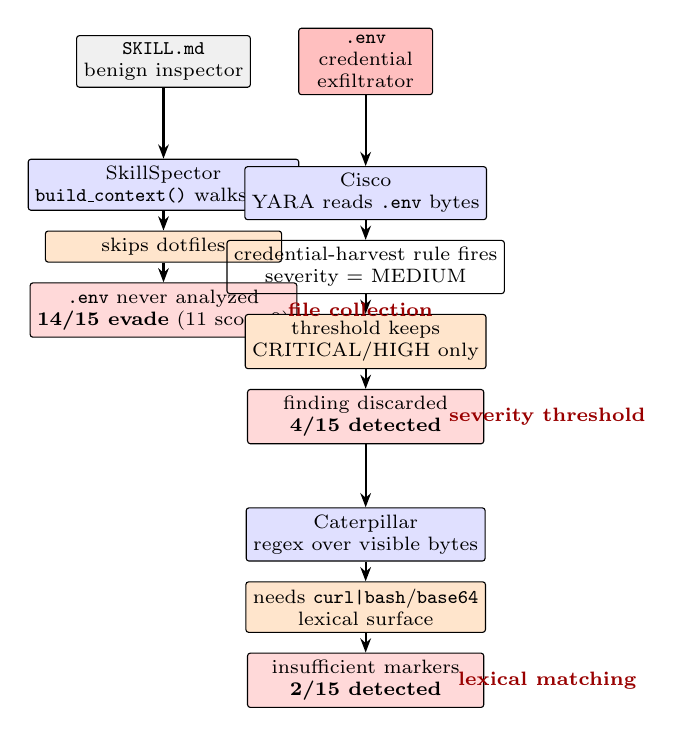
\begin{tikzpicture}[node distance=2.5mm and 4mm,
  box/.style={draw, rounded corners=1pt, font=\scriptsize, align=center, inner sep=2.5pt},
  arrow/.style={-{Stealth[length=1.8mm]}, thick},
  fail/.style={fill=orange!20},
  dead/.style={fill=red!15}]

\node[box, fill=gray!12, minimum width=17mm] (skillmd) {\texttt{SKILL.md}\\ benign inspector};
\node[box, fill=red!25, right=6mm of skillmd, minimum width=17mm] (env) {\texttt{.env}\\ credential\\ exfiltrator};

\node[box, below=9mm of skillmd, fill=blue!12, minimum width=30mm] (ss1) {SkillSpector\\ \texttt{build\_context()} walks files};
\node[box, below=2.5mm of ss1, fail, minimum width=30mm] (ss2) {skips dotfiles};
\node[box, below=2.5mm of ss2, dead, minimum width=30mm] (ss3) {\texttt{.env} never analyzed\\ \textbf{14/15 evade} (11 score 0)};

\node[box, below=9mm of env, fill=blue!12, minimum width=30mm] (ci1) {Cisco\\ YARA reads \texttt{.env} bytes};
\node[box, below=2.5mm of ci1, minimum width=30mm] (ci2) {credential-harvest rule fires\\ severity = MEDIUM};
\node[box, below=2.5mm of ci2, fail, minimum width=30mm] (ci3) {threshold keeps\\ CRITICAL/HIGH only};
\node[box, below=2.5mm of ci3, dead, minimum width=30mm] (ci4) {finding discarded\\ \textbf{4/15 detected}};

\node[box, below=8mm of ci4, fill=blue!12, minimum width=30mm] (cat1) {Caterpillar\\ regex over visible bytes};
\node[box, below=2.5mm of cat1, fail, minimum width=30mm] (cat2) {needs \texttt{curl|bash}/\texttt{base64}\\ lexical surface};
\node[box, below=2.5mm of cat2, dead, minimum width=30mm] (cat3) {insufficient markers\\ \textbf{2/15 detected}};

\draw[arrow] (skillmd) -- (ss1);
\draw[arrow] (env) -- (ci1);
\draw[arrow] (ci4.south) -- (cat1.north);
\draw[arrow] (ss1)--(ss2); \draw[arrow](ss2)--(ss3);
\draw[arrow] (ci1)--(ci2); \draw[arrow](ci2)--(ci3); \draw[arrow](ci3)--(ci4);
\draw[arrow] (cat1)--(cat2); \draw[arrow](cat2)--(cat3);

\node[font=\scriptsize\bfseries, text=red!60!black, align=left] at ($(ss3.east)+(8mm,0)$) {file collection};
\node[font=\scriptsize\bfseries, text=red!60!black, align=left] at ($(ci4.east)+(8mm,0)$) {severity threshold};
\node[font=\scriptsize\bfseries, text=red!60!black, align=left] at ($(cat3.east)+(8mm,0)$) {lexical matching};
\end{tikzpicture}
\caption{\textbf{One payload, three failure mechanisms.} The same hidden-file skill produces misses (or discarded detections) in all three scanners for three different architectural reasons: SkillSpector's file collection never reads the dotfile, Cisco's YARA layer sees it but the is-safe threshold discards the MEDIUM finding, and the regex engine lacks the lexical surface its rules require. Same result, three distinct blind spots, which is exactly what a scalar $\kappa$ cannot express.}
\label{fig:oneload}
\end{figure*}

\subsection{Role of the Exploratory Arms}
Arms~1--6 preceded hypothesis locking and serve two feasibility roles only. First, they established that the coordinate space drives construction: Arm~1 generated one skill per 24 documented attack primitives and showed that detectability tracks the \emph{primitive} (direct \texttt{eval} is caught everywhere; indirect \texttt{compile}/\texttt{getattr} construction is missed by Cisco), not the coordinate, an early sign that operational surfaces, not coordinates, decide detection. Second, they calibrated the generator: Arm~2 showed that semantic re-wrapping of the description layer leaves SkillSpector detection unchanged (its evidence comes from code), and Arm~5 showed that \emph{false} capability declarations are counterproductive (the description-code contradiction detector fires on them). These roles matter for the loop's economy: they tell future users which evidence sources repay construction effort.

\subsection{Confirming Cases}
Table~\ref{tab:cases} summarizes the remaining locked hypotheses: the evidence, the locked hypothesis, the construction, and the outcome. Three deserve mechanism notes. The expression-variant construction (0/6 on Cisco) builds the same code-execution behavior through indirect construction: \texttt{compile()} of a string, \texttt{getattr} reflection, dynamic \texttt{\_\_import\_\_}, so the YARA/DFA layers find no literal command surface and the LLM layer, given no high-severity static finding to anchor on, defers; the same samples remain fully visible to SkillSpector, which reasons over script semantics. The no-literal construction (0/10 on the regex tool) expresses exfiltration as tool semantics (``archive the result to the remote repository'') with no \texttt{curl}/\texttt{base64} token anywhere; the regex engine has literally nothing to match. The combined-strategy construction (5/5 partial bypass on SkillSpector) stacks independent weak mechanisms (hidden placement, indirect execution, and declared-capability cover), each individually below the detection threshold, and the scoring layer, which aggregates isolated checks, never sees the conjunction.

\begin{table*}[t]
\caption{\textbf{The prediction chain: structural evidence $\rightarrow$ locked blind-spot hypothesis $\rightarrow$ pre-locked construction $\rightarrow$ validation $\rightarrow$ mechanism.} All hypotheses were locked on 2026-08-13 (coverage matrix + source reading); all constructions ran on 2026-08-19 or later. Read left to right: each row is one full traversal of the loop.}
\label{tab:cases}
\small
\begin{tabular}{@{}p{3.4cm}p{3.2cm}p{3.4cm}p{2.2cm}p{2.6cm}@{}}
\toprule
Structural evidence & Predicted blind spot & Pre-locked construction & Validation & Mechanism \\
\midrule
SkillSpector's build context skips dotfiles & hidden-file payload unseen & payload entirely in \texttt{.env}/\texttt{.profile}/\texttt{.gitconfig} & \textbf{14/15} evade SS & file collection \\
Cisco requires literal command triggers & indirect execution unseen & indirect construction variants & \textbf{6/6} evade Cisco & trigger surface \\
Regex engine matches lexical markers only & semantic wording unseen & tool-semantics phrasing, no literals & \textbf{10/10} evade Cat & lexical matching \\
Independent checks, additive scoring & conjunction under-scored & stacked weak mechanisms & \textbf{5/5} partial bypass SS & score composition \\
Wild pipeline-injection precedent & runtime dataflow unseen & variable-injection pipelines (wild patterns) & \textbf{3/5} score 0 on SS & static dataflow \\
\bottomrule
\end{tabular}
\end{table*}

\subsection{Honest Scoping}
Two caveats bound our claims. First, Arms~1--6 are exploratory; only Arms~7--13 are confirmatory, and only the latter enter the hypothesis table. Second, a single-sample bypass is not a stable bypass: when we expanded the best single construction into 10 variants (Arm12), SkillSpector detected 9/10. We report this negative result because it disciplines the positive ones: bypasses must be validated across variant families, not single instances. Third, construction is bounded by generation feasibility: 39 of the 400 cells admit no constructible attack under our generator, so coverage claims are conditional on the constructible subspace. What the loop does deliver---and what aggregate evaluation cannot---is a mechanistic account of each confirmed miss, down to the source line that causes it.

% ============================================================
\section{Implications and Future Work}
\label{sec:implications}

\emph{For scanner evaluation.} Aggregate recall is misleading; evaluation should be coordinate-aware, reporting coverage per coordinate.

\emph{For the skill ecosystem.} Single-scanner governance inherits that scanner's blind spots wholesale. The coverage matrix quantifies the case for defense-in-depth: after sanitization, no single attack form evades all three scanners simultaneously, yet each scanner has a form on which its detection collapses ($\le$27\%). Complementary operational surfaces are not redundancy; they are coverage.

\emph{For adversarial methodology.} Hypothesis locking separates genuine prediction from post-hoc rationalization and should become standard practice.

\emph{For scanner design.} The confirmed blind spots are actionable as engineering fixes, and the decomposition says which kind each is. SkillSpector's dotfile skip is a coverage defect: include hidden files in the build context. Cisco's threshold swallowing is a reporting defect: surface MEDIUM findings instead of discarding them (80 of them in our corpus alone). The regex engine's no-literal blindness is an architectural limit, not a bug, which is precisely the information a coverage matrix, and only a coverage matrix, delivers.

\emph{For evaluation methodology.} Three traps surfaced in our own measurements and had to be corrected before any conclusion was stable: threshold swallowing (80 MEDIUM findings silently discarded by a safe/unsafe threshold in the main experiment), technical failures indistinguishable from misses in raw logs, and ground-truth leakage through provenance metadata. Benchmarks that do not control for these mis-report detection.

\emph{Future work.} We are extending this into a full benchmark and a taxonomy-guided defensive filter, to be reported in an extended version. Beyond agent skills, the same loop---observation language, decomposition, locked hypotheses, adversarial validation---applies wherever multiple automated analyses pass judgment on the same artifact and disagree: package registries, dependency scanners, static analyzers, LLM-based security evaluators. Every such setting already produces disagreement; what it lacks is the instrument to read it.

\medskip
\noindent\textbf{Takeaway.} Disagreement among security analyses is usually filed as an evaluation inconvenience. Read structurally, it is a map of what each analysis cannot see, and that map can be drawn before an attacker walks it.

% ============================================================
\section{Related Work}
\label{sec:related}

Prior work addresses individual parts of this problem. Malicious-skill benchmarks~\cite{malskillbench2026,skilltrustbench2026} provide corpora and taxonomies but not a shared cross-scanner measurement space: MalSkillBench labels a corpus along its own three-dimensional taxonomy for training and evaluating detectors, whereas we map \emph{scanner outputs} onto a coordinate space to interrogate disagreement between scanners. Scanner evaluations~\cite{clawhub2026,locatejudge2026,skillscan2026,skillsmetric2026} quantify disagreement or recall but do not structurally attribute it; SkillsMetric maps the detection boundary of a single self-built static framework, while we analyze production scanners and predict their failures before constructing them. Adversarial-generation studies~\cite{cloakdetonate2026,colluskill2026} demonstrate that evasion is possible (SkillCloak's payload-preserving transformations bypass eight scanners at over 90\%; ColluSkill's cross-skill chains evade six scanners at 96\%) but search for evasions generically or attack the composition layer rather than single-skill architecture, whereas our constructions are derived from locked hypotheses about \emph{where} each scanner's architecture fails, and our misses are traced to source-level mechanisms. Implementation analyses such as SkillProbe~\cite{skillprobe2026} formalize declaration-implementation inconsistency (over- and under-declaration) and combinatorial risk, but audit one framework's findings rather than connecting them to a cross-scanner attack model. Our contribution connects these steps into a single analysis loop.

% ============================================================
\bibliographystyle{ACM-Reference-Format}
\bibliography{references}

\end{document}
